\documentclass[../../../../main.tex]{subfiles}
\begin{document}

\begin{flushright}
\footnotesize\textit{【自動文字起こし・要確認】}
\end{flushright}

\noindent
[\textbf{解}] $l, g$ の単位方向ベクトルを $\vec{l}, \vec{g}$ とする. 又 点 $X$ の位置ベクトルをその小文字で表す. $\alpha, \beta$ を実数として ($0 < \alpha < \beta$)
\begin{align*}
\vec{a_2} &= \vec{a_1} + \alpha \vec{l} \\
\vec{a_3} &= \vec{a_1} + \beta \vec{l} \\
\vec{b_2} &= \vec{b_1} + \alpha \vec{g} \\
\vec{b_3} &= \vec{b_1} + \beta \vec{g}
\end{align*}
とかけるから
\begin{align*}
\vec{m_2} &= \frac{\vec{a_1} + \vec{b_1}}{2} + \frac{\alpha}{2}(\vec{l} + \vec{g}) \\
\vec{m_1} &= \frac{\vec{a_1} + \vec{b_1}}{2} \\
\vec{m_3} &= \frac{\vec{a_1} + \vec{b_1}}{2} + \frac{\beta}{2}(\vec{l} + \vec{g})
\end{align*}
となる. つまり $M_1, M_2, M_3$ は方向ベクトル $\vec{l} + \vec{g}$ とし, $M_1$ を通る直線上にある.

\begin{center}
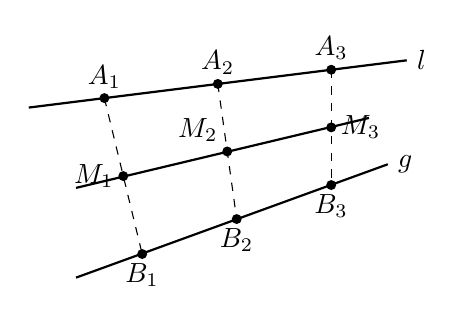
\begin{tikzpicture}[scale=1.2, >=stealth]
  \draw[thick] (0, 2) -- (4, 2.5) node[right] {$l$};
  \draw[thick] (0.5, 0.2) -- (3.8, 1.4) node[right] {$g$};

  \coordinate (A1) at (0.8, 2.1);
  \coordinate (A2) at (2.0, 2.25);
  \coordinate (A3) at (3.2, 2.4);

  \fill (A1) circle (1.5pt) node[above] {$A_1$};
  \fill (A2) circle (1.5pt) node[above] {$A_2$};
  \fill (A3) circle (1.5pt) node[above] {$A_3$};

  \coordinate (B1) at (1.2, 0.45);
  \coordinate (B2) at (2.2, 0.82);
  \coordinate (B3) at (3.2, 1.18);

  \fill (B1) circle (1.5pt) node[below] {$B_1$};
  \fill (B2) circle (1.5pt) node[below] {$B_2$};
  \fill (B3) circle (1.5pt) node[below] {$B_3$};

  \draw[dashed] (A1) -- (B1);
  \draw[dashed] (A2) -- (B2);
  \draw[dashed] (A3) -- (B3);

  \coordinate (M1) at (1.0, 1.275);
  \coordinate (M2) at (2.1, 1.535);
  \coordinate (M3) at (3.2, 1.79);

  \fill (M1) circle (1.5pt) node[left] {$M_1$};
  \fill (M2) circle (1.5pt) node[above left] {$M_2$};
  \fill (M3) circle (1.5pt) node[right] {$M_3$};

  \draw[thick] (0.5, 1.15) -- (3.6, 1.89);
\end{tikzpicture}
\end{center}

\newpage

\end{document}
